\documentclass[a4paper]{report}

%====================== PACKAGES ======================

\usepackage[french]{babel}
\usepackage[utf8x]{inputenc}
%pour gérer les positionnement d'images
\usepackage{float}
\usepackage{amsmath}
\usepackage{graphicx}
\usepackage[colorinlistoftodos]{todonotes}
\usepackage{url}
%pour les informations sur un document compilé en PDF et les liens externes / internes
\usepackage{hyperref}
%pour la mise en page des tableaux
\usepackage{array}
\usepackage{tabularx}
%pour utiliser \floatbarrier
%\usepackage{placeins}
%\usepackage{floatrow}
%espacement entre les lignes
\usepackage{setspace}
%modifier la mise en page de l'abstract
\usepackage{abstract}
%police et mise en page (marges) du document
\usepackage[T1]{fontenc}
\usepackage[top=2cm, bottom=2cm, left=2cm, right=2cm]{geometry}
%Pour les galerie d'images
\usepackage{subfig}

%====================== INFORMATION ET REGLES ======================

%rajouter les numérotation pour les \paragraphe et \subparagraphe
\setcounter{secnumdepth}{4}
\setcounter{tocdepth}{4}



%======================== DEBUT DU DOCUMENT ========================

\begin{document}

%régler l'espacement entre les lignes
\newcommand{\HRule}{\rule{\linewidth}{0.5mm}}

%page de garde
\begin{titlepage}
\begin{center}

% Upper part of the page. The '~' is needed because only works if a paragraph has started.

\includegraphics[width=0.35\textwidth]{./logo}~\\[1cm]

%\textsc{\LARGE Université ou Entreprise}\\[1.5cm]

\textsc{\Large }\\[0.5cm]

% Title
\HRule \\[0.4cm]

{\huge \bfseries \\ Découverte du framwork Apache OFBiz.
Dévéloppement d'une API HTTP, basé le sur style architectural REST et inégration dans un contexte de projet client. \\[0.4cm] }

\HRule \\[1.5cm]

% Author and supervisor
\begin{minipage}{0.4\textwidth}
\begin{flushleft} \large
\emph{Auteur:}\\
Artemiy \textsc{Rozovyk}\\

\end{flushleft}
\end{minipage}
\begin{minipage}{0.4\textwidth}
\begin{flushright} \large
\emph{Tuteur de stage:} \\
Mathieu \textsc{Lirzin}\\
\emph{Référent:} \\
Florent \textsc{Foucaud}
\end{flushright}
\end{minipage}

\vfill

% Bottom of the page
{\large \today}

\end{center}
\end{titlepage}
%ne pas numéroter cette page
\newpage
\tableofcontents
\newpage


\renewcommand{\abstractnamefont}{\normalfont\Large\bfseries}
%\renewcommand{\abstracttextfont}{\normalfont\Huge}

\renewcommand{\abstractname}{Remerciements}
\addcontentsline{toc}{chapter}{Remerciements}
\begin{abstract}
	Je tiens tout d'abord à remercier mon tuteur de stage, Mathieu Lirzin, pour les conseilles et les savoir-faire qu'il a partagé avec moi tout au long de mon stage. 
	\\
	
	De même, je remercie à Pierre Gaudin et à Antoine Ouvrard, pour leur collaboration et leur aide au cours des projets qu'on a pu développer ensemble. 
\\

	Enfin, merci à toute l’équipe de Néréide, pour leur accueil, leurs temps consacré à moi et leur bonne humeur constante.	
\end{abstract}

\newpage




%espacement entre les lignes d'un tableau
\renewcommand{\arraystretch}{1.5}

%====================== INCLUSION DES PARTIES ======================


%recommencer la numérotation des pages à "1"


\chapter{Introduction}

Intro\footnotemark\\
Intro2\footnotemark\\
%note en bas de page
\iffalse
\section{Sujet}

Bla(cf. fig. 1.1)\\

%inclusion d'une mage dans le document
\begin{figure}[!h]
\begin{center}
%taille de l'image en largeur
%remplacer "width" par "height" pour régler la hauteur
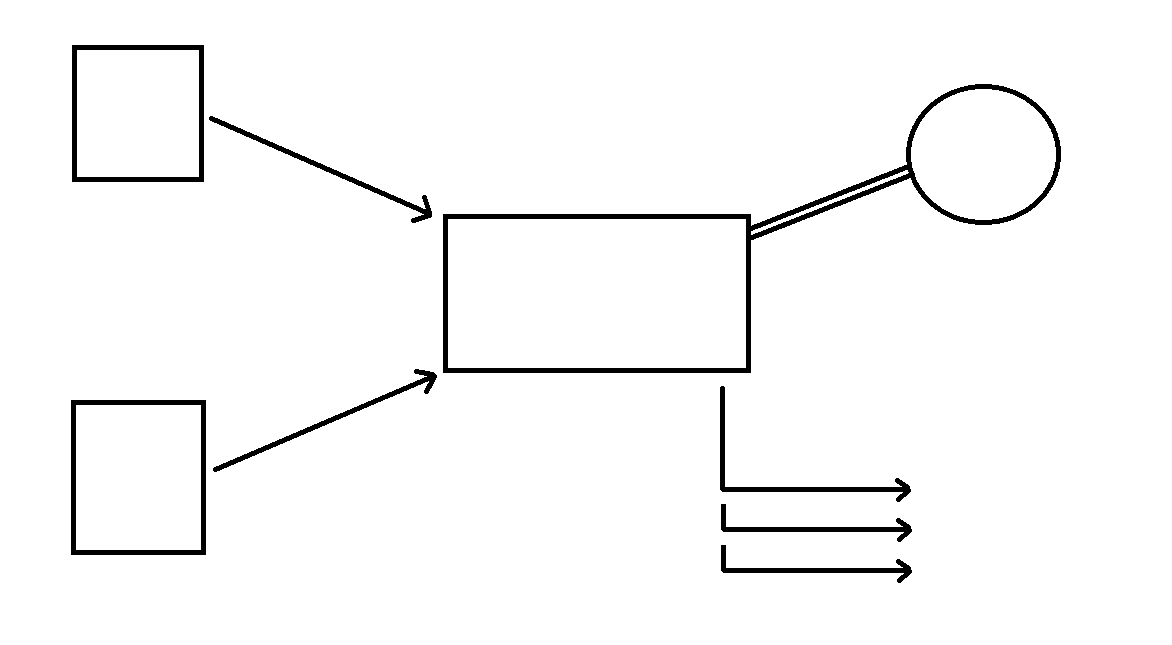
\includegraphics[width=15cm]{presentation/schema}
\end{center}
%légende de l'image
\caption{Schéma descriptif}
\end{figure}

%Contenu de la note précédemment marquée avec \footnotemark
\footnotetext{Note bas de page "intro"}

Bla
%retour à la ligne (alinea)

Bla\\
%saut de paragraphe

Bla

\newpage

\section{Problématique soulevée}

Bla

\begin{center}
Problématique du sujet
\end{center}

\section{Hypothèse de solution}

%Quoi :
Bla\\

Voici une liste :
\begin{itemize}
\item item 1;
\item item 2;
\item item 3;
\item item 4.
\end{itemize}

Bla\\

%Comment :
Bla

Bla\footnotemark\\

%Detail :
Bla(cf. ref. \cite{cite6}).
%citation référencé dans le document "bibliographie.bib" inclus à la fin du document
\fi
\footnotetext{Note bas de page "bla"}
\footnotetext{dog2}

\chapter{Contexte du stage}

Intro

\section{Entreprise}
\subsection{Presentation générale }
SCOP Situé à Tours...

\subsection{Domaine}
Retail
\subsection{Activité}
Dévéloppement spécifique 
Maintenance et support applicatif
Administration système
\subsection{Projets}

\section{L'architecture de OFBiz}
\subsection{Vue d'ensemble sur l'architecture}
DSL en XML, servlettes, jdbc ...
\subsection{Composants }

\subsection{Container}
\subsection{Web applications}
\subsection{Entity engine}
\subsection{Service engine}
\subsection{Screen engine}
\subsection{Fonctionnel métier}
\subsection{Lien avec les connaissences obtenu lors de la formation universitaire}
\subsubsection{MVC}
\subsubsection{Servlet}
\subsubsection{FreeMarker -JSP}
\subsubsection{Notion d'entié - Symfony}
\subsubsection{Routage}

\section{Sujet de stage }



\subsection{API REST au sein d'OFBiz}
\iffalse
Bla


Voici un tableau (cf. fig. 2.1) récapitulatif de notre analyse de l'existant...\\

%tableau centré à taille variable qui s'ajuste automatiquement suivant la longueur du contenu
\begin{figure}[!h]
\begin{center}
\begin{tabular}{|l|l|l|l|l|}
  \hline
  Solution & Critère 1 & Critère 2 & Critère 3 & Critère 4\\
  \hline
  Solution 1(cf. ref. \cite{cite0}) & Oui & Oui & Oui & Oui \\
  Solution 2(cf. ref. \cite{cite1}) & Oui & Oui & Oui & Non \\
  Solution 3(cf. ref. \cite{cite2}) & Oui (sauf telle chose) & Non & Non & Oui\\
  Solution 4(cf. ref. \cite{cite3}) & Oui& Non & Oui & Non\\
  Solution 5(cf. ref. \cite{cite4}) & Oui (uniquement ceux-ci) & Non & Oui & Non\\
  \hline
\end{tabular}
\end{center}
\caption{Tableau récapitulatif des solutions}
\end{figure}
\fi

 
\chapter{Analyse des besoins}

Intro

\section{Besoins fonctionnels}

Après une analyse des besoins fonctionnels du projet, nous avons défini deux sous catégories. D'un côté, les besoins [...], de l'autre, les besoins [...].

\subsection{Sous-partie 1}

Bla

\subsection{Sous-partie 2}

Bla

\newpage

\section{Besoins non-fonctionnels}

Comme précédemment, nous avons choisi de distinguer deux catégories pour les besoins non-fonctionnels. D'une part, nous avons les besoins non-fonctionnels pour les [...], et d'autre part ceux pour [...]. Nous avons aussi pris en compte les contraintes de développement, que nous détaillerons à la fin de cette partie.

\subsection{Sous-partie 1}

Bla\\

Aperçu du rendu souhaité :

\begin{figure}[!h]
\begin{center}
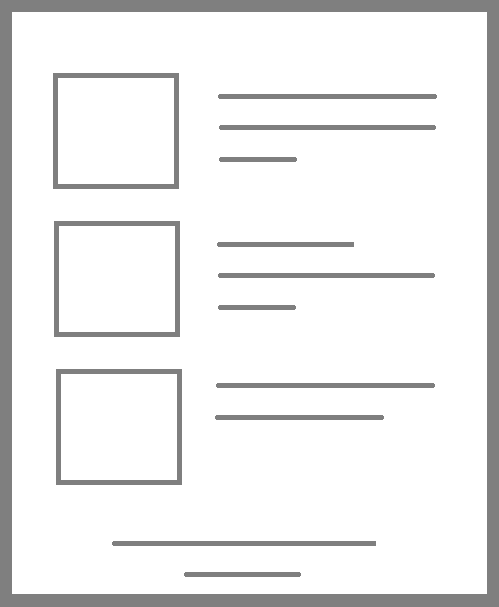
\includegraphics[height=10cm]{besoins/rendu}
\end{center}
\caption{Rendu attendu}
\end{figure}

\subsection{Sous-partie 2}

Bla

\newpage

\section{Développement}

Intro

\subsection{Tâches}

Bla\\


%tableau à taille fixée sur certaines colonnes (param sur la ligne \begin{tabularx}, voir wiki pour plus d'info sur la syntaxe
\begin{figure}[!h]
\begin{center}
\begin{tabularx}{17cm}{|c|p{6cm}|X|}
  \hline
  Priorité & Nom & Raison\\
  \hline
  1 & Tache 1 & Doit être vérifié en premier car sinon [...] \tabularnewline
  2 & Tache 2 & On doit pouvoir [...] \tabularnewline
  3 & Tache 3 & Comme les principales fonctionnalités permettant de tester sont opérationnelles, nous pouvons passer à cette tâche. \tabularnewline
  4 & Tache 4 & Parce que [...] \tabularnewline
  5 & Tache 5 & La tache 5 fait partie des principales [...]. \tabularnewline
  6 & Tache 6 & Dernière fonctionnalité essentielle à mettre en place. \tabularnewline
  7 & Tache 7 & Non-essentiel, mais apporterait un plus au projet. \tabularnewline
  8 & Tache 8 & Non-essentiel, mais apporterait un plus au projet. \tabularnewline
  \hline
\end{tabularx}
\end{center}
\caption{Tableau récapitulatif des tâches}
\end{figure}

\subsection{Tests}

Bla\\

\begin{figure}[!h]
\begin{center}
\begin{tabularx}{17cm}{|p{6cm}|X|}
  \hline
  Fonctionnalité & Test\\
  \hline
  Fonction 1 & Quand [...], vérifier [...]. \tabularnewline
  & Et quand [...], vérifier [...]. \tabularnewline
  Fonction 2 & Vérifier [...]. \tabularnewline
  Fonction 3 & Vérifier [...]. \tabularnewline
  Fonction 4 & Avoir [...]. \tabularnewline
  Fonction 5 & Accéder à [...]. \tabularnewline
   & Vérifier que [...]. \tabularnewline
  Fonction 6 & Accéder à [...]. \tabularnewline
   & Et vérifier [...]. \tabularnewline
  Fonction 7 & Installer [...]. \tabularnewline
   & Vérifier [...]. \tabularnewline
  Fonction 8 & Compter [...]. \tabularnewline
  \hline
\end{tabularx}
\end{center}
\caption{Tableau récapitulatif des tests}
\end{figure}
\iffalse
\chapter{Conclusion}
\ganttset{%
	calendar week text={%
		\pgfcalendarmonthshortname{\startmonth}~\startday%
	}%
}
\newganttlinktype{f-m}{
	\ganttsetstartanchor{on right=1}
	\ganttsetendanchor{on left=0}
	\draw[/pgfgantt/link]
	([xshift=-.2pt]\xLeft, \yUpper) --       % xshift to fit arrow
	node[pos=.5, /pgfgantt/link label node] {\ganttlinklabel} 
	(\xRight, \yLower);
}
\setganttlinklabel{f-m}{}

	\begin{ganttchart}[
		hgrid,
		vgrid={*1{blue!30},
			 *6{black,dotted},
			 *1{red!30},
			 *2{black,dotted},
			 *1{blue!30},
			 *{34}{black,dotted},
		 	 *1{green!30},
	 	 	 *1{red!30},
 	 	 	 *{10}{black,dotted},
  	 	 	 *1{green!30}},
		x unit=3mm,
		time slot format=isodate,
		inline,
		bar/.append style={fill=blue!37},
	    group/.append style={draw=black, fill=black!50},
		milestone/.append style={fill=green, rounded corners=6pt,scale=2},
		milestone inline label node/.append style={right=1mm},
	]{2019-03-28}{2019-05-25}
	\gantttitlecalendar{year, month=name, week} \\
	\ganttgroup{Analyse des besoins}{2019-03-29}{2019-04-7}\\
	\ganttgroup{Réalisation technique}{2019-04-5}{2019-05-13}\\
	\ganttgroup{Maintenance}{2019-05-13}{2019-05-24} \\
	\ganttbar{OFBiz}{2019-04-01}{2019-04-11}\\
	\ganttbar[
	bar/.append style={ fill=red!50
	}]{REST}{2019-04-08}{2019-04-28} \\
	\ganttbar[
	bar/.append style={ fill=orange!50
	}]{Entitymaint}{2019-04-20}{2019-05-12} \\

	\ganttmilestone{Preuve de concept}{2019-05-12}] \\
	\ganttbar[
	bar/.append style={ fill=purple!40, dashed
	}]{Revue de code}{2019-05-13}{2019-05-23} \\
	\ganttlink{elem3}{elem4}
	\ganttlink{elem4}{elem5}
	\ganttlink[link type=f-m]{elem5}{elem6}
	\ganttlink[link type=dr]{elem4}{elem6}
	\ganttlink[link type=f-m]{elem6}{elem7}
	\end{ganttchart}

\chapter{Résultats}

\section{Partie 1}

Intro

\subsection{Sous-partie 1}

\paragraph*{Paragraphe 1 (n'apparaitra pas dans l'index)} Bla

\paragraph*{Paragraphe 2} Bla

\paragraph*{Paragraphe 3} Bla

\subsection{Sous-partie 2}

Bla

\subsection{Sous-partie 3}

Bla

\section{Partie 2}

Intro

\subsection*{Sous-partie 1 ('apparaitra pas dans l'index)} Bla

\paragraph*{Paragraphe 1 ('apparaitra pas dans l'index)} Bla

\paragraph*{Paragraphe 2} Bla

\paragraph*{Paragraphe 3} Bla

\newpage

\subsection*{Sous-partie 2}

Bla

%galerie d'image
\begin{figure}[htp]
  \centering
  \subfloat[Première image]{\label{fig:première}
\includegraphics[scale=0.8]{resultats/gallerie}}
  ~ %espace entre deux images sur une même ligne
  \subfloat[Deuxième image]{\label{fig:deuxième}
\includegraphics[scale=0.8]{resultats/gallerie}}
  ~
  \subfloat[Troisième image]{\label{fig:troisième}
\includegraphics[scale=0.8]{resultats/gallerie}}
  ~\\ %saute une ligne dans la galerie d'image
  \subfloat[Quatrième image]{\label{fig:quatrième}
\includegraphics[scale=0.8]{resultats/gallerie}}
  ~
  \subfloat[Cinquième image]{\label{fig:cinquième}
\includegraphics[scale=0.8]{resultats/gallerie}}
  \caption{Différents screenshots quelque chose, en gallerie}
  \label{fig:gallerie1}
\end{figure}

\chapter{Bilan}

%Rappel du context
Intro / Rappel Contexte

Nous avons donc pu en tirer la problématique suivante :

\begin{center}
\hskip7mm
Problématique du sujet
\end{center}

Bla

Bla\\

Bla\\

%Rappel des résultats
Bla

Bla\\

Bla

Bla

\newpage

%Conclusion/Perspectives
Bla

Bla\\

Bla

%Ne pas numéroter cette partie
\part*{Annexes}
%Rajouter la ligne "Annexes" dans le sommaire
\addcontentsline{toc}{part}{Annexes}

\chapter*{Annexe 1}
\addcontentsline{toc}{chapter}{Annexe 1}

%changer le format des sections, subsections pour apparaittre sans le num de chapitre
\makeatletter
\renewcommand{\thesection}{\@arabic\c@section}
\makeatother

%recommencer la numérotation des section à "1"
\setcounter{section}{0}

Intro

\section{Partie 1}

Bla

\subsection{Sous-partie 1}

Bla

\subsection{Sous-partie 2}

Bla

\subsection{Sous-partie 3}

Bla

\section{Partie 2}

Bla

\subsection{Sous-partie 1}

Bla

\subsection{Sous-partie 2}

Bla

\subsection{Sous-partie 3}

Bla

\chapter*{Annexe 2}
\addcontentsline{toc}{chapter}{Annexe 2}

%recommencer la numérotation des section à "1"
\setcounter{section}{0}

Intro

\section*{Prérequis}
\addcontentsline{toc}{section}{Prérequis}

Bla

\begin{itemize}
\item item1;
\item item2;
\item item3;
\item item4.
\end{itemize}

Bla

\section{Partie 1}

Bla

\subsection{Sous-parie 1}

Bla

\subsection{Sous-parie 2}

Bla

\section{Partie 2}

\begin{center}
\textsc{Attention !}

\textit{Texte d'avertissement}
\end{center}

Bla

\newpage

\section{Partie 3}

Bla

\begin{figure}[!ht]
\begin{center}
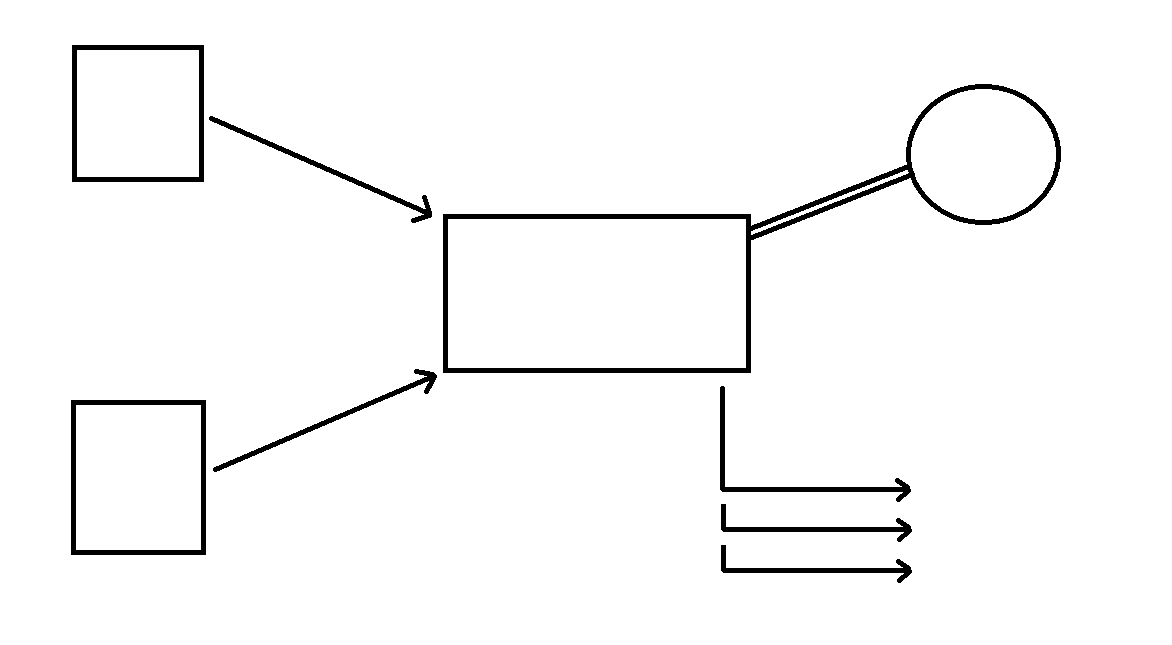
\includegraphics[height=8cm]{presentation/schema}
\end{center}
\caption[schema]{Presentation schema}
\end{figure}

\paragraph*{Paragraphe 1}
~\\
\hskip7mm

Bla

\paragraph*{Paragraphe 2}
~\\
\hskip7mm

Bla

\paragraph*{Paragraphe 3}
~\\
\hskip7mm

Bla
\fi
\newpage

%récupérer les citation avec "/footnotemark"
\nocite{*}

%choix du style de la biblio
\bibliographystyle{plain}
%inclusion de la biblio
\bibliography{bibliographie.bib}
%voir wiki pour plus d'information sur la syntaxe des entrées d'une bibliographie

\end{document}